\documentclass[conference]{IEEEtran}
\IEEEoverridecommandlockouts
% The preceding line is only needed to identify funding in the first footnote. If that is unneeded, please comment it out.
\usepackage{cite}
\usepackage{amsmath,amssymb,amsfonts}
\usepackage{algorithmic}
\usepackage[ruled, linesnumbered]{algorithm2e}
\usepackage{graphicx}
\usepackage{textcomp}
\usepackage{xcolor}
\usepackage{hyperref}
\usepackage{multirow}
\usepackage{subfig}

\usepackage{fancyhdr} 
\lhead{\textit{Inverse Reinforcement Learning Tool for MiniGrid environment}}
\rhead{\textit{HCI 2019/2020}}
\cfoot{\thepage}
\pagestyle{fancy} 

\hypersetup{colorlinks=true, linkcolor=blue, urlcolor=magenta, citecolor=red}
\def\BibTeX{{\rm B\kern-.05em{\sc i\kern-.025em b}\kern-.08em
    T\kern-.1667em\lower.7ex\hbox{E}\kern-.125emX}}
    
\def\BibTeX{{\rm B\kern-.05em{\sc i\kern-.025em b}\kern-.08em
    T\kern-.1667em\lower.7ex\hbox{E}\kern-.125emX}}
    
\begin{document}

\title{Inverse Reinforcement Learning Tool\\for MiniGrid environment
}

\author{\IEEEauthorblockN{Giulio Bazzanti, Niccol\'o Biondi}
\IEEEauthorblockA{\textit{Dipartimento di Ingegneria dell'Informazione (DINFO)} \\
University of Florence, Florence, Italy\\
giulio.bazzanti@stud.unifi.it, niccolo.biondi1@stud.unifi.it}
}

\maketitle
% Nicco
\begin{abstract}
In this paper we explore the effectiveness of an Inverse Reinforcement Learning (IRL) system to define an agent able to reach the goal state in MiniGrid Gym environment.
To do that, we define a reward model that exploits preferences between short segments of agent trajectories (clips) to provide rewards to the policy model instead of the environment ones. These preferences are collected by our IRL tool, that is a GUI that we develop for an user who wants to annotate pairs of clips. 

With our experiments we force the agent to follow a sub-optimal trajectory in the MiniGrid Empty 6x6 environment. We also study how the reward model gives the reward to the policy model and why its loss grows during our training protocol. 
\end{abstract}

\begin{IEEEkeywords}
Inverse Reinforcement Learning, Human Computer Interaction, MiniGrid Gym
\end{IEEEkeywords}


\section{Introdution}
Reinforcement Learning (RL) is an area of machine learning concerned with how a particular artificial agent makes several actions inside an environment in order to maximize some cumulative rewards. With this kind of technique, the agent has the possibility to learn the right behavior to adopt in a certain environment through the \textsl{trial-and-error} mechanism. To achieve these goals, a policy network (the agent behavior) is defined and it takes the current environment state to perform the best action in the environment. Nowadays, the RL achieves superhuman performance in a range of environments, but requires that a designer manually specify a reward function.

In the Inverse Reinforcement Learning (IRL), the policy does not receive the reward directly from the environment during the training process. Instead,  we assume that there is a human in the loop who has an intention for the agent’s task, and communicates this intention to the agent using one the preferences feedback channel.  If the policy model mimics the human expert’s behavior well, it can achieve the performance of the human on the task. In this project, we implement the Inverse Reinforcement Learning method described in\ \cite{NIPS2018_8025} to train a policy agent to achieve the goal in the \textsl{Minigrid} environment\ \cite{gym_minigrid}. We use this kind of simple environment because, unlike is described in the original algorithm, we don't use a set of human demonstrations provided by an expert to pretrain the policy. In our case we use only the preferences, the human labels\ \cite{NIPS2018_8025}, provided by the user to define a reward model function which will give rewards for policy training. This choice allows us to train simultaneously the policy and the reward model. 
The human labels are collected thanks to a simple application, where the user can specify his preference between pairs of small segments of agent trajectories.
 
 In video games, the RL is used to define the Non-Player Characters (NPCs), that sometimes have superhuman abilities, overcoming the player skills. On the other hand, the RL can produce a predictable NPCs, making the game experience boring. So, in these cases, the players will not be involved in the game, abandoning it. 
 
 The scope of our project is to propose an IRL tool with which the video game designers can control the NPCs (agents) behaviour in order to create more interactive and engaging video games.
 
     % Bazza
\section{Inverse Reinforcement Learning}\label{IRL}

To understand better the aim of Inverse Reinforcement Learning, we describe firstly what Reinforcement Learning is.

In a way, Reinforcement Learning is the science of making optimal decisions using experiences. Breaking it down, the process of Reinforcement Learning involves these simple steps: the agent takes from the environment the current state; it computes the best action; the agent performs it in the environment. The goal of RL is to find an optimal behavior strategy for the agent to obtain optimal rewards.
The main idea behind the RL approach is the \textsl{Markov decision process}. This process is defined by a tuple $( S, A, R, p, \gamma)$:

\begin{equation}\label{eq:Markov}
     p(s', r | s, a) = Pr[ S_{t+1} = s', R_{t+1} = r | S_{t} = s, A_{t} = a ] 
\end{equation}

\begin{equation}\label{eq:discounted}
    G_{t} = R_{t+1} + \gamma R_{t+2} + {\gamma}^2 R_{t+3} + \dots
\end{equation}
     


 where $S_{t}, S_{t+1} \in S$ are the states, $A_{t+1} \in A$ is an action, $R_{t}, R_{t+1} \in R$ are the rewards, p is the process dynamism and $G_{t}$ is the discounted reward. The discounted rewards indicates to the agent the best trajectory to achieve the goal. \\
 The Markov decision process \ref{eq:Markov}, in other words, defines the transition probability in a new state, taking some rewards from the current state with the execution of an action. 
Another important component is the discount factor $\gamma$. It defines the penalty to uncertainty of future rewards, so larger $\gamma$ increases the sensibility to the future rewards.
This coefficient value is in $(0,1)$, but typically is close to $1$.

In the RL is defined a \textsl{policy network} that implements the agent. This policy network $\pi$ define an actions probability distribution given the states:

\begin{equation}
    \pi( A_{t} = a | S_{t} = s), \forall A_{t} \in A, S_{t} \in S
\end{equation}

This creates a \textsl{trajectory}, that is an ordered sequence of states, actions and rewards: $S_{0}, A_{0}, R_{1}, S_{1}, A_{1}, R_{2}, S_{2}, A_{2}, R_{3} \dots$.
The agent, therefore, tends to maximize the "expected" reward following the policy network $\pi$. To do that, the policy is modeled with a parameterized function respect to $\theta$. This function is  $\pi_{\theta}(a|s)$ and it represents the probability of performing the action \textit{a} given the state \textit{s}. \\ 
We can now define the \textsl{Reinforcement Learning Objective}: maximize the "expected" reward following a parameterized policy:

\begin{equation}
    J(\theta) = E_{\pi_{\theta}} [r(\tau)]
\end{equation}

where $r(\tau)$ define the \textsl{total reward} for a given trajectory $\tau$. \\
A standard method to find the $\theta$ that it is an optimum for J is the \textsl{Gradient Ascent} method. Here $\theta$ is updated like that:

\begin{equation}
    \theta_{t+1} = \theta_{t} + \alpha\nabla_{\theta} J(\theta)
\end{equation}

Using gradient ascent, we can move $\theta$ toward the direction suggested by the gradient $\nabla_{\theta}J(\theta)$ to find the best $\theta$ for $\pi_{\theta}$ that produces the highest return. Computing the gradient $\nabla_{\theta}J(\theta)$ is tricky because it depends on both the action selection and the stationary distribution of states following the target selection behavior \cite{gradient}. The only problem is that since the environment is unknown, it is difficult to estimate the effect on the state distribution by a policy update.
For this reason, it is used the \textsl{Policy Gradient Theorem} which simplify the gradient computation  $\nabla_{\theta}J(\theta)$:

\begin{equation}\label{eq:nablae}
    \nabla E_{\pi_{\theta}}[r(\tau)] = E_{\pi_{\theta}}[r(\tau)\nabla log(\pi_{\theta}(\tau))]
\end{equation}

where:

\begin{equation}\label{eq:pitau}
    \pi_{\theta}(\tau) = P(s_{0}) + \prod_{t=1}^{T} \pi_{\theta}(a_{t}|s_{t})p(s_{t+1}, r_{t+1} | s_{t}, a_{t})
\end{equation}

In equation \ref{eq:pitau}, \textit{P} represents the \textsl{ergodic distribution} which starts from some state $s_{0}$. 

Every step, an action \textit{a} is taken according to $\pi_{\theta}$ and, based on that, the environment dynamic \textit{p} decides which state transition has to be performed. Then this is multiplied by the trajectory length T. Now consider the logarithm of equation \ref{eq:pitau}, we have that $\log\pi_{\theta}(\tau)$ is:

\begin{equation*}
    \log P(s_{0}) + \sum_{t=1}^{T} \log\pi_{\theta}(a_{t}|s_{t}) + \sum_{t=1}^{T} \log p(s_{t+1},r_{t+1}|s_{t}, a_{t}) 
\end{equation*}

from which we can see that:

\begin{equation}\label{eq:nablalog}
    \nabla \log\pi_{\theta}(\tau) = \sum_{t=1}^{T}\nabla\log\pi_{\theta}(a_{t}|s_{t})
\end{equation}

Now putting together the equations\ \ref{eq:nablae} and\ \ref{eq:nablalog}, we obtain the final policy gradient algorithm:

\begin{equation}\label{eq:policygradient}
    \nabla E_{\pi_{\theta}}[r(\tau)] = E_{\pi_{\theta}}[r(\tau)(\sum_{t=1}^{T} \nabla \log\pi_{\theta}(a_{t}|s_{t})]    
\end{equation}

Replacing $r(\tau)$ from the equation\ \ref{eq:policygradient} with the discounted rewards $G_{t}$\ (\ \ref{eq:discounted}), we obtain the classic policy gradient algorithm called \textit{Reinforce} (\textit{Monte-Carlo Policy Gradient}):

\begin{equation}
    \nabla E_{\pi_{\theta}}[r(\tau)] = E_{\pi_{\theta}}[\sum_{t=1}^{T} G_{t} \nabla \log\pi_{\theta}(a_{t}|s_{t})] 
\end{equation}

In IRL, the policy does not receive the reward directly from the environment. Instead,  we assume that there is a human in the loop who has an intention for the agent's task, and it communicates this intention to the agent using one feedback channel, that is the Preferences\ \cite{NIPS2018_8025}. The preferences are pairs of short trajectory segments of agent's behavior which the human compares, preferring those that are closer to the intended goal.
The preferences are collected during the experiment while the policy is training. 
In this case, are introduced two new actors: an \textit{annotator} and a \textit{reward model}. The former gives preference feedback; the latter estimates a reward function from the annotator's preferences which will give rewards to the policy during its training.
              % Bazza
\section{Method}\label{method}

In this section we describe our method, that follows the one adopted in \cite{NIPS2018_8025}.

\subsection{Training Protocol}\label{Alg}
In IRL has to be defined three basic components: the \textit{policy} that specify how the agent moves in the environment; an \textit{annotator} which gives preferences to clips; and a \textit{reward model} that estimates a reward function from the provided preferences. 

The training phase of our system follows the protocol described in the Algorithm\ \ref{alg:train_proto}, where the policy and the reward model are jointly trained.

\begin{algorithm}
\caption{Training Protocol}
\label{alg:train_proto}
\SetAlgoLined
\begin{algorithmic}[1]
\STATE Run the policy in the environment and store "initial trajectories".
\STATE The annotator annotated all the "initial clips" and create the annotation buffer.
\STATE Pretrain the reward model from the annotation buffer.
\FOR{\textit{M} epochs} 
\STATE Train the policy in the environment for \textit{N} episodes with rewards from the reward model.
\STATE Sample pairs of clips from the resulting trajectories.
\STATE The annotator labels the selected pairs and puts them in the annotation buffer.
\STATE Train the reward model for \textit{K} batches from the annotation buffer.
\ENDFOR 
\end{algorithmic}
\end{algorithm}
 
We achieve our best configuration with $N=150$ policy episodes and $K=1500$ reward model batches. %at the $21^{st}$ iteration

The number of sampled clips decreases as the number of epochs increases. In particular the annotator labels the $100\%$ of clips at first iteration and, every 5 iterations, that percentile decreases by $20\%$. 
\subsection{Policy}
During the training of the policy, the agent interacts with the environment over a number of time steps (that we set to a maximum of T = 150). In time step $t$ the agent receives an observation $o_t$ from the environment and takes an action $a_t$. This action is chosen with a sampling of a Categorical distribution where the logits are the output values of the policy model giving $o_t$. A trajectory is the set of couples ${(o_1, a_1), (o_2, a_2), \ldots, (o_T, a_T)}$. If the agent reaches the goal state in a step $\textit{t}<T$, we terminate this episode before the agent has done all the steps.

Typically in Reinforcement Learning the agent receives a reward $r_t$ at each step from the environment, but in Inverse Reinforcement Learning the reward model plays this role. The advantage consists of providing the agent non-zero rewards before reaching the environment goal. The Minigrid reward function give non-zero reward only in the environment goal.
Furthermore, in complex environment, the agent spends a lot of steps to reach the goal and to learn the environment rules because of sparse rewards. The reward model, instead, provides dense rewards to the agent from the begging of its episodes. 

Our policy model is inspired to the one presented in \cite{karpathy}, this is a fully connected layer with 64 hidden units and ReLU activation followed by another fully connected layer with 7 output units (that are clamped from -1000, 1000). The input to the model are the agent observations at each agent step. 

For our experiments we adopt Adam optimizer with $0.0001$ of learning rate and we regularize that with $0.01$ of weight decay. 

\subsection{Annotator}
The aim of the annotator is to give preference feedback about segments of agent trajectory, called \textit{clip}. A clip consists of 5 consecutive agent trajectory's elements $\{(o_i, a_i)_{i=t}^{t+4}\}$. Since the trajectory can have variable dimension (e.g. when the agent reaches the environment goal), we create a clip generator able to create clips of a fixed length from a trajectory. If the agent reaches the environment goal during this trajectory at time stamp $t$, with $t \mod T \not= 0$, our generator creates the last clip with the goal state replicated several times in order to create another clip with the same length.

After the clips generation, the annotator has to label pairs of sampled clips. In our experiments the sampling is uniform and without bootstrapping. The only possible values for a single preference provided by the annotator are $(1,0)$, $(0,1)$, $(0.5,0.5)$ or $(0,0)$. In the first two chances, the annotator prefers one clip with respect to the other; when the preference is $(0.5,0.5)$ we got two \textit{indifferent labels}; the last possibility refers to a discarded couple of clips, that will be deleted from the training process. The indifferent labels match to two clips where it's impossible to give a preference feedback, and those annotations produced an unusual result: the more their number is, the more the reward model loss will be. For more details about that, please refer to Section \ref{05}.

The annotator has to force the agent to take a specific route in the environment, and to reach that goal we have to annotate only clips with agent steps in that direction. Even if, in a clip, the agent takes only one step in one position that is not in this direction, we reject the clip. 

In this paper we analyze two different types of preference feedback: those provided by a human annotator, and those given by an artificial one, that we call Oracle. Human preferences are collected by our IRL Tool, described in Section \ref{04}, where we support the user during the annotation process with a GUI. Instead, the Oracle gives preferences based on handcrafted rules.

The result of the annotation process is the annotation buffer, that is a set of triples $\{(\sigma^1_i, \sigma^2_i, \mu_i)\}$, where $\sigma^1, \sigma^2$ are two clips and $\mu$ represents the provided preference. We reset the annotation buffer each iteration of the training protocol (see Algorithm\ \ref{alg:train_proto}) and we never put the discarded pairs of clips ($\mu=(0,0)$) in the annotation buffer.


\subsection{Reward Model}
The reward model $\hat{r}$ is a preference predictor, its target is to emulate how the annotator labels each pair of clips. To achieve this goal, it is assumed that the annotator's probability of preferring a segment $\sigma^i$ depends exponentially on the value of the reward summed over the length of the segment\ \cite{NIPS2018_8025}:
\begin{equation}
    \hat{P}[\sigma^1 \succ \sigma^2] = \frac{exp(\sum_{o \in \sigma^1} \hat{r}(o))}{exp(\sum_{o \in \sigma^1} \hat{r}(o) + \sum_{o \in \sigma^2} \hat{r}(o))}
\end{equation}

%%%%%%%%%%%%%%%%%%%%%%%%%%%%%%%%%%%%%%%%%%%%%%%%%%%%%%%%%%%%%%%%%%%%%%%%%%%%%%%%%%%%%%%%%%%%%%
\begin{figure*}[t]
    \qquad
	\subfloat{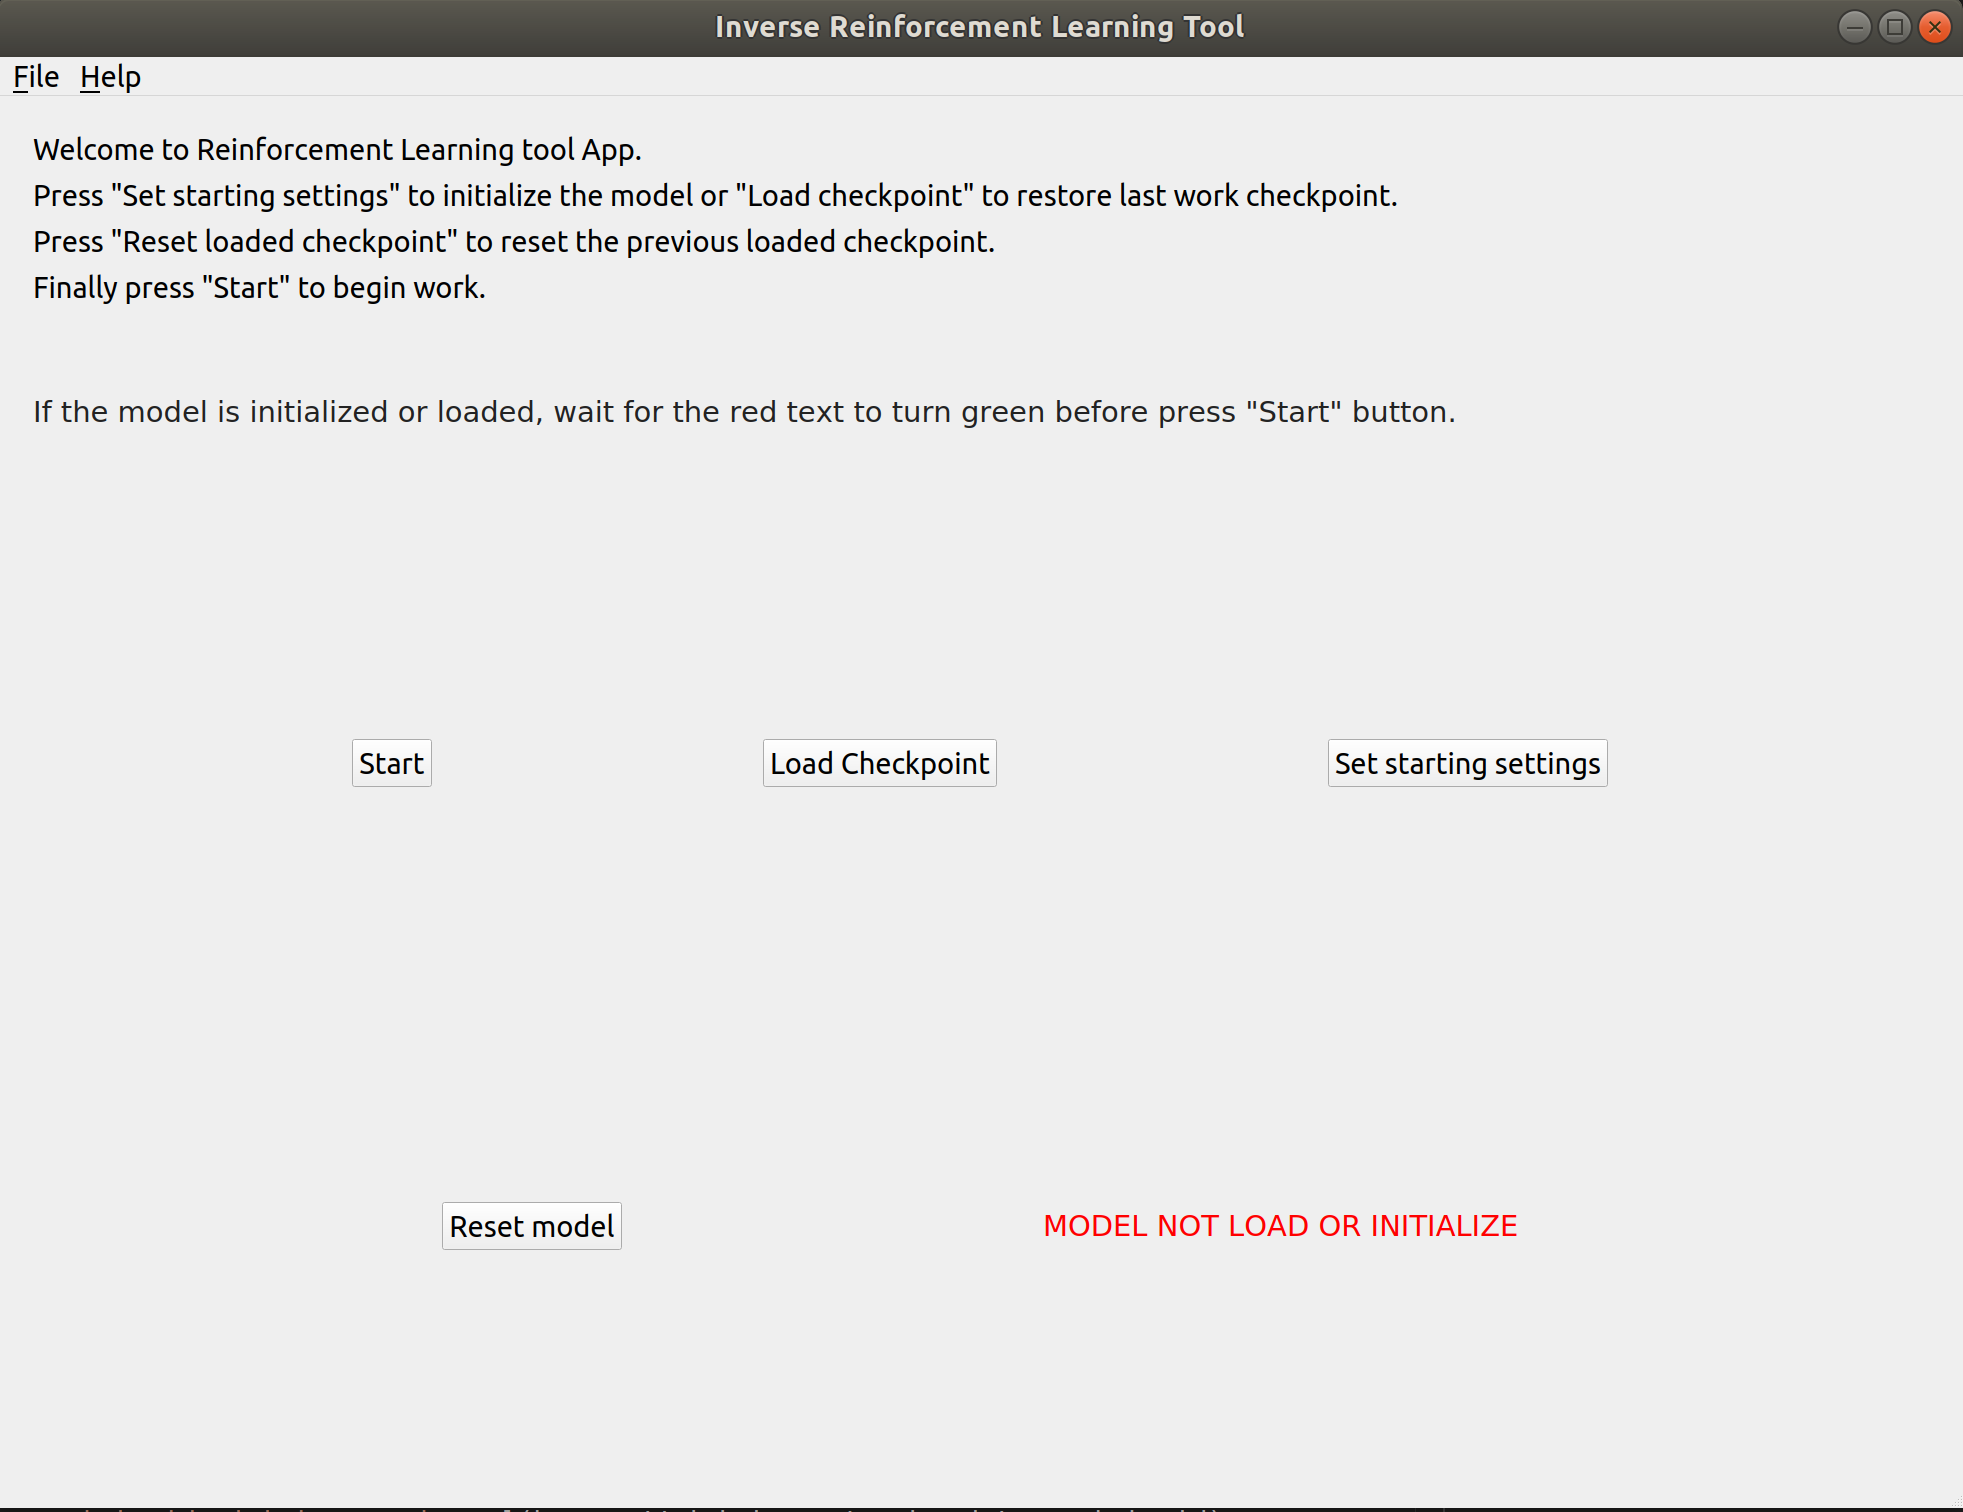
\includegraphics[width=0.30\linewidth]{data/main_view.png} }%
	\subfloat{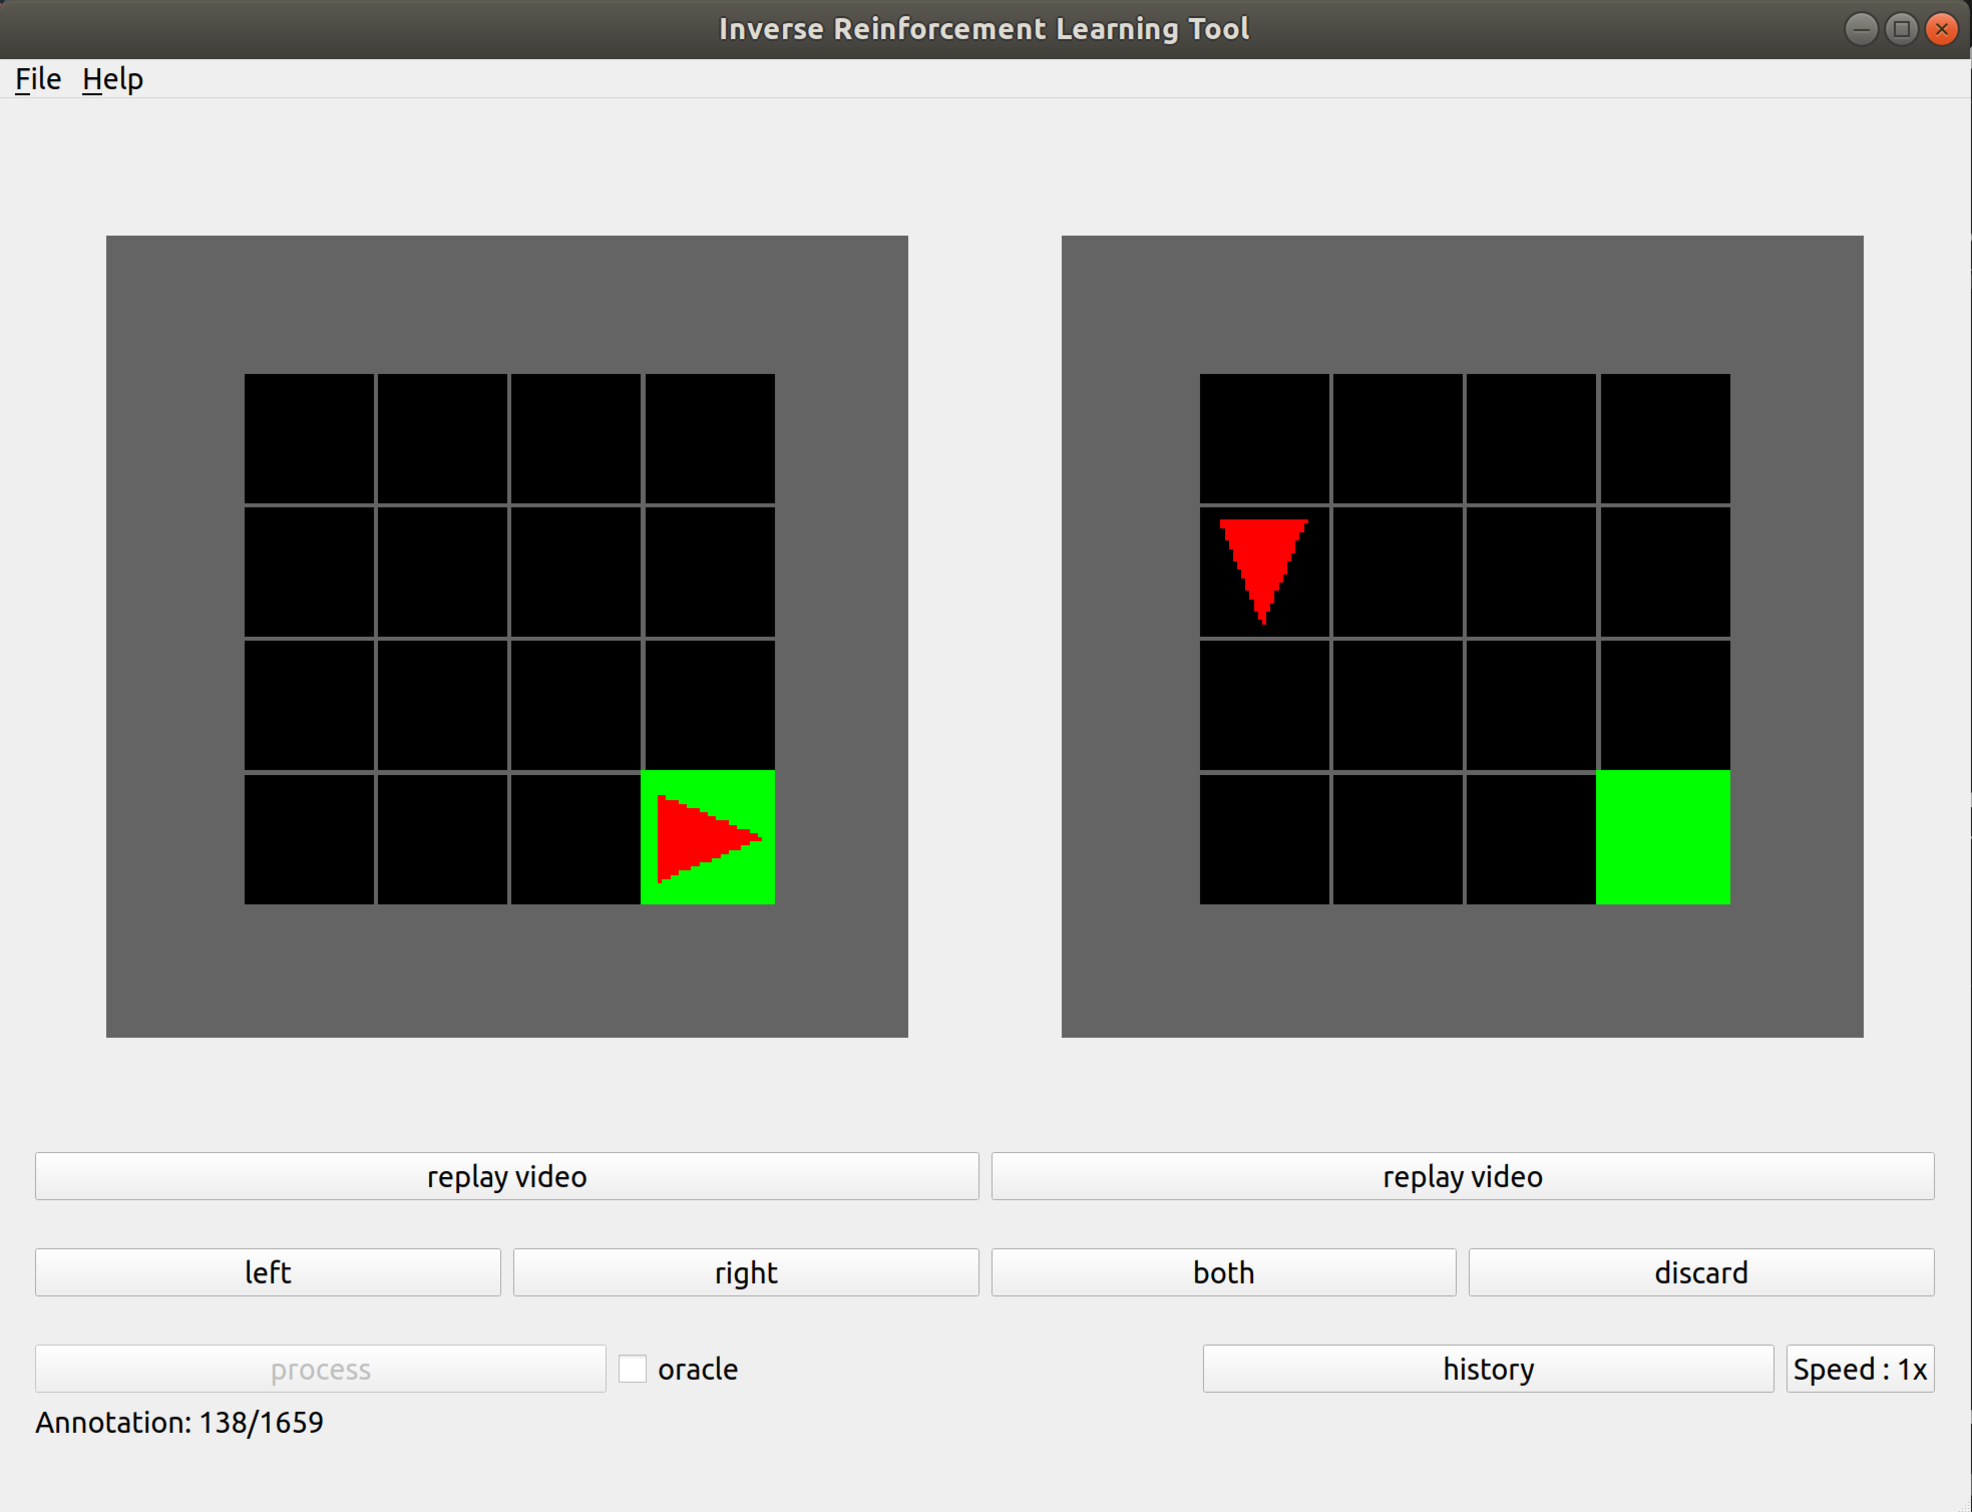
\includegraphics[width=0.30\linewidth]{data/alg_view.png} }%
	\subfloat{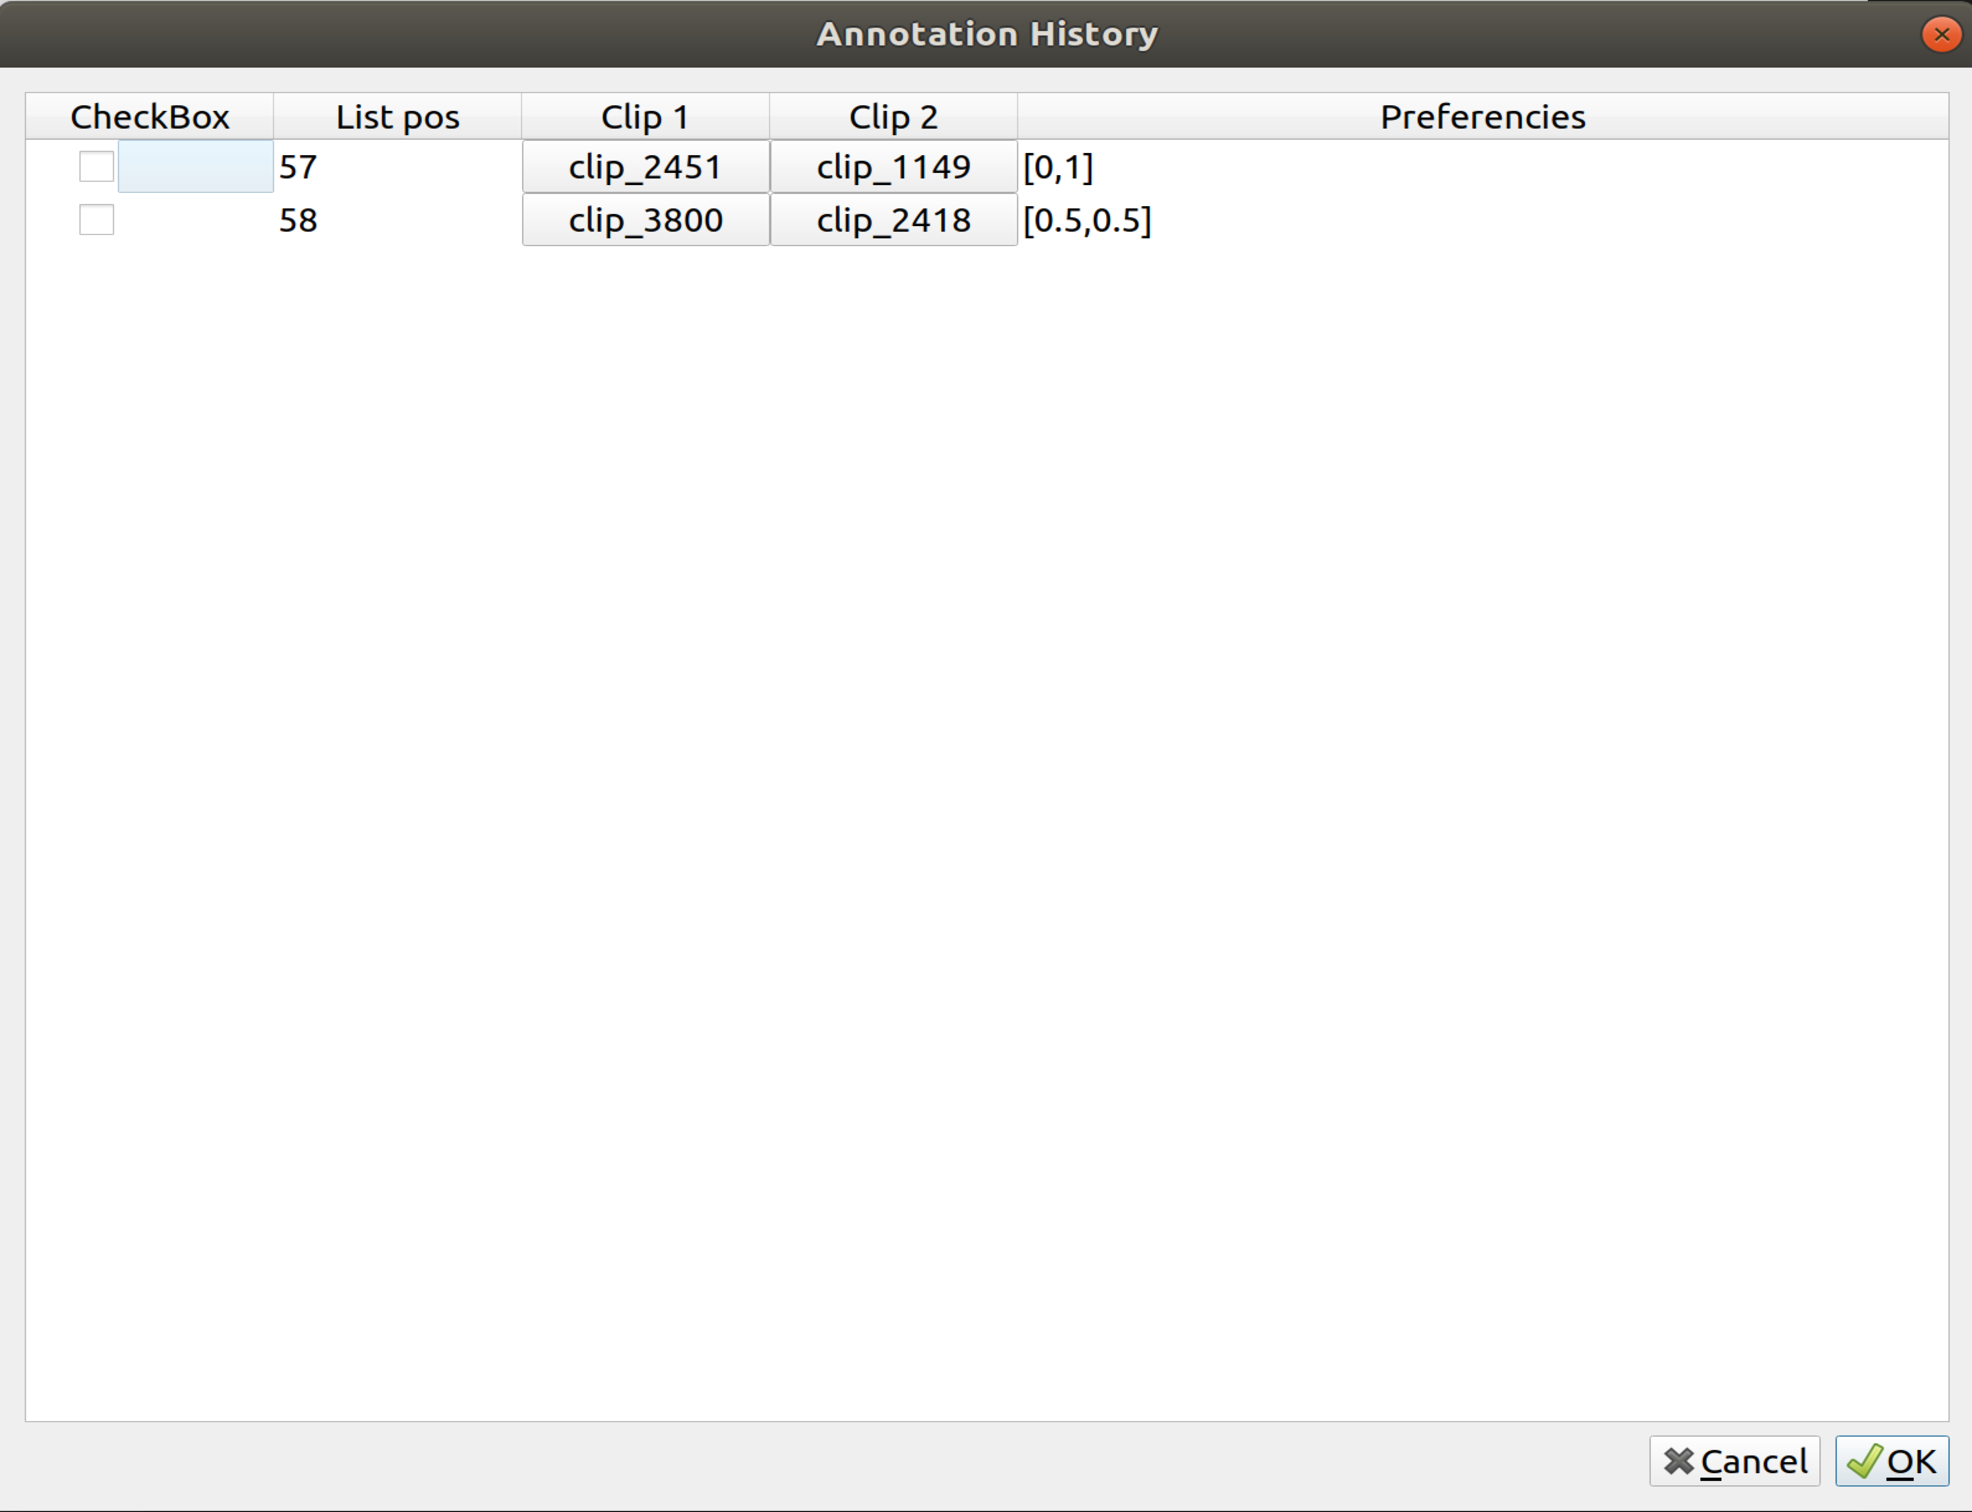
\includegraphics[width=0.30\linewidth]{data/history_window.png} }%
	\caption{Different application views. The first is the Main Window, that is the configuration panel. The second represent the implementation of the training protocol, that supports the annotation process. The last window is the History Panel.}%
	\label{fig:Application}%
\end{figure*}
%%%%%%%%%%%%%%%%%%%%%%%%%%%%%%%%%%%%%%%%%%%%%%%%%%%%%%%%%%%%%%%%%%%%%%%%%%%%%%%%%%%%%%%%%%%%%%%

So the reward model $\hat{r}$ is trained to minimize the cross-entropy loss between these predictions and the actual judgment labels:
\begin{equation}\label{eq:rewardloss}
    loss(\hat{r}) = - \sum_{(\sigma^1,\sigma^2,\mu)\in A} \mu(1)log(\hat{P}_{1,2}) + \mu(2)log(\hat{P}_{2,1})
\end{equation}
where $\hat{P}_{i,j} = \hat{P}[\sigma^i \succ \sigma^j]$. This follows \cite{10.1093/biomet/39.3-4.324}, where is described how to estimate score function from pairwise preferences. Since the reward model is trained on an annotation buffer A relatively small (100-200 triples), we use L2 regularization during the optimization process (with $\lambda = 0.01$). Furthermore, we standardize the output of the reward model over the last 300 predicted rewards to have 0 mean and 0.5 standard deviation (those are empirical values, see Section \ref{05} for more details).

Our reward model is a MLP net with two fully connected layers: the first with 64 hidden units and ReLU activation and the second with one output unit without any activation function. For our experiments we adopt Adam optimizer with $0.0003$ of learning rate.

The input to the model are two clips $\sigma^1$ and $\sigma^2$ both composed by 5 consecutive agent observations. For each clip we compute the output of the model, that is a list of 5 rewards, one for each agent state present in the processed clip. 

During the training phase, the reward model performs over the annotation buffer K batches each consisting of 16 sampled triples with bootstrapping, because of the small dimensions of the training set. 

           % Nicco 


\section{IRL Tool}\label{04}

In this section we present a simple application which include the IRL process described in Section\ \ref{method}, with which the user can easily express his preferences between pairs of clips and change them if they are not correct.
To train the reward model the human has to create an annotation buffer where inside there are all the preferences the human made. A preference is a tuple $( \sigma^1, \sigma^2, \mu)$, where $\sigma^1, \sigma^2$ represent the short trajectory segments of agent's behavior and $\mu$ defines the human preference between the two clips (that can be $(1, 0)$, $(0, 1)$, $(0, 0)$ and $(0.5, 0.5)$). 

When the application starts, the user sees the main view, that is represented in the left image in Figure\ \ref{fig:Application}.
In this window, he can decide to load a previous session, tapping the "Load Checkpoint" button or starting a new one session, tapping the "Set starting setting" button, where he has to set all the system hyper-parameters. Anyway, after clicking the "Start" button, the tool changes window, the central picture of Figure\ \ref{fig:Application}. Here the user can start the IRL process described in Algorithm\ \ref{alg:train_proto} tapping the button "process".
To improve the user experience, we connect each training iteration to the click of this button: the number of clicks that the user made corresponds to the number of epochs (M).

We also include the first three steps of the Algorithm\ \ref{alg:train_proto} in the main loop. At epoch $0$ the policy creates the "initial trajectories" used to pretrain the reward model. To speed up this process, the application saves the reward model weights in a folder specifying the adopted environment and the reward model hyper-parameters. In this way, if the user will start new IRL project with same configurations for the environment and the reward model, our application will load these weights, skipping the reward model pretrain.

With the IRL tool, the user also decides to label manually the clips or not. Selecting the oracle check button, the application will give artificial preferences trough an Oracle. Instead the human labeling is supported with the display of the current clips and with the "left", "right", "discard" and "both" buttons. Depending on which button he clicks, we give to this pair of clips the corresponding label (respectively $(1, 0)$, $(0, 1)$, $(0, 0)$, $(0.5, 0.5)$) and we put that in the annotation buffer. 

The user can check his last preferences in the History window, presented in the right picture of Figure\ \ref{fig:Application}. With this feature, he can look again the clips and decide if the given preferences are correct or not. If not he can select the wrong ones and label them again.

Finally, we consider to include saving methods: auto-save and manual ones. The former is made in the three main step of the Algorithm\ \ref{alg:train_proto}: during the policy training, during the annotation and at the end of the reward model training. The latter is achieved when the user click "Save State" in the File menu. In this case, the user can specify the folder where he wants to save the current system state. This is composed by the current policy and reward model weights and by the annotation buffer state (the user preferences). However, in both the saving methods, the tool do not save the system state during the reward model training, but only at the beginning and the end of that.       % Bazza








\section{Experimental results}\label{05}
In this section we present all the obtained results of our experiments. First of all we report our attempts on tuning the system components: policy, annotator and reward model. We also explore different kind of Oracle that we exploit to train faster our system, since with only human annotations the training time would have been longer. Finally we underline the grown of reward model loss.




\subsection{Hyper-parameters Tuning}        % Setting IRL components
We implement an IRL system which include three principal components: a policy, an annotator and a reward model. Our aim is to force the agent to achieve the goal trough the left bottom corner of the map, for a total of 9 agent steps (one more step with respect to the optimal goal trajectory).

Each iteration the policy makes 150 episodes each one composed by 150 agent steps. The dimension of an episode is an important value, since, in order to converge, it's essential that the agent reaches the goal as often as possible in the first iterations of the training process. 


%%%%%%%%%%%%%%%%%%%%%%%%%%%%%%%%%%%%%%%%%%%%%%%%%%%%%%%%%%%%%%%%%%%%%%%%%%%%%%%%%%%%%%%%%%%%%%%
\begin{figure}[t]
    \centering
    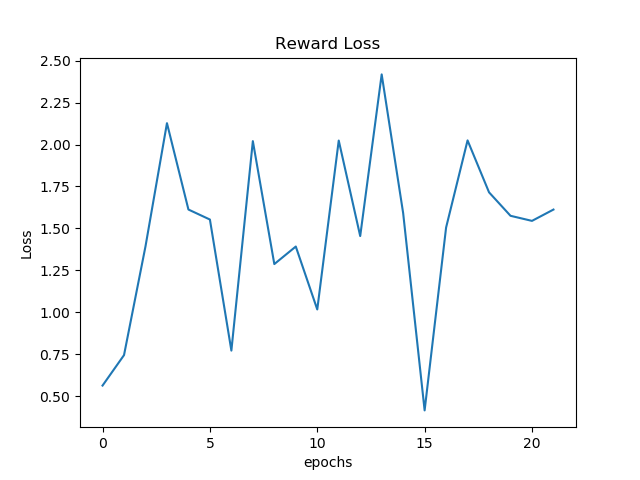
\includegraphics[width=\linewidth]{data/reward_loss.png} 
    \caption{Reward model loss with early stop after 25 iterations.}
	\label{fig:rewardloss}%
\end{figure}
%%%%%%%%%%%%%%%%%%%%%%%%%%%%%%%%%%%%%%%%%%%%%%%%%%%%%%%%%%%%%%%%%%%%%%%%%%%%%%%%%%%%%%%%%%%%%%%

In Inverse Reinforcement Learning the policy does not take rewards from the environment but from the reward model, that is trained to assign a reward $r\in R$ to each agent state. Since the reward model is trained only comparisons (like we described in section \ref{method}), we perform a standardization, with $0$ mean and $0.5$ of std, on the reward model output, because it's scale-free. The std value is empirical and it has a huge impact on the system's performance: larger values of it imply bigger rewards in every agent step, while smaller ones often result in negative goal reward. In the first iterations, the majority of clips show the agent in the upper part of the map trying to learn some environment rules. This involves that the reward model does not learn nothing about the bottom states, especially the goal state. So the agent learns different environment rules respect to the ones that we want to teach him.
When we set std to 1 or surrounding values, the agent learned to stand still, since the upper states provide him higher rewards. In the other scenario, when std is about 0.05 (like the authors of \cite{NIPS2018_8025} adopted in their work), rewards got a so small range of possible values that the agent receive a negative reward in the goal state. Thus we find that values between $0.5$ and $0.6$ are the best choices for std of agent rewards. 
The standardization is performed on the last 300 agent step rewards, two episodes approximately, that allow us to compute the right values' range comparing same agent action distributions.

%%%%%%%%%%%%%%%%%%%%%%%%%%%%%%%%%%%%%%%%%%%%%%%%%%%%%%%%%%%%%%%%%%%%%%%%%%%%%%%%%%%%%%%%%%%%%%%
\begin{figure}[t]
    \centering
    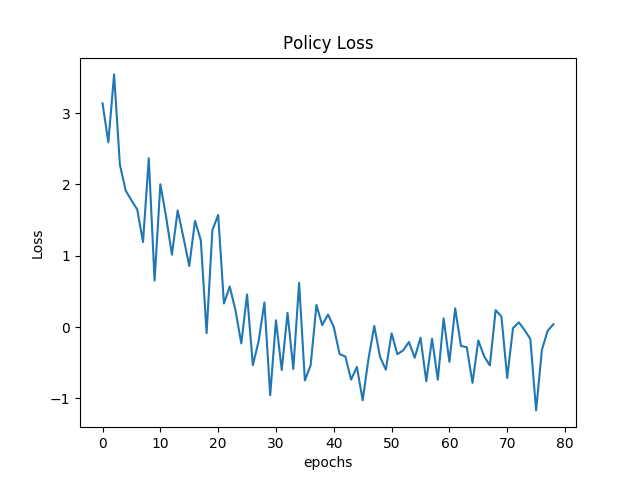
\includegraphics[width=\linewidth]{data/policy_loss_80.png} 
    \caption{Policy model loss after 80 training iterations.}
	\label{fig:losspolicy}%
\end{figure}
%%%%%%%%%%%%%%%%%%%%%%%%%%%%%%%%%%%%%%%%%%%%%%%%%%%%%%%%%%%%%%%%%%%%%%%%%%%%%%%%%%%%%%%%%%%%%%%

We set the clip length to 5. We choose that value because we want to force a trajectory of 9 agent steps. 
For this reason with length of 5, clips are big enough to show if the agent is computing movements in the trajectory we wanted to teach him, or not. The result is that the "perfect trajectory" is composed by two clips. The first where the agent turns down, runs across the left part of the map and, again, turns towards the goal. In the second the agent simply goes forward until its destination, that need just 4 moves. For this reason the corresponding clip will have the goal state replicated twice. 

Our experiments are carried out with an Oracle, that gives preferences regarding handcrafted rules. To define this, we have to generate a matrix that corresponds to the environment structure where each position has its reward. Our aim is that the reward model will learn this Oracle matrix from the annotations without ever seeing it. In particular, we explore different types of that artificial annotator, one where there are smoother values of matrix, and another matrix with sparse values. Both of them have reward 1 in each state of the trajectory that we want to force to the agent, and 10 as the goal reward. The difference between the two versions are in the rewards of the other states that are not in this trajectory. 
The sparse Oracle has 0 as reward for all these states, while the smooth Oracle sets those rewards according with the following rule: $r_{i,j}=max(reward_{k,l})/2, k\in\{i-1,i,i+1\}, j\in\{j-1,j,j+1\}$. 
However we report our best results with the sparse artificial annotator, because with the other our agent learned different routes with respect to the only one we want to teach him.  

The reward model hyper-parameters need to be tuned as well as the other, even if they are not so crucial like other parameters. We achieved our best results with  K, the number of reward model batches, set to $1500$. In other experiments we try to set a flexible value to K according to the dimension of the annotation buffer, in essence every iteration we compute K as \textit{len(annotation\_buffer)}$\cdot10$. We also study the effect of changing the percentile of annotated clip with which we train the reward model. Every 5 epoch we decrease this percentile by $20\%$ from a maximum of $100\%$ to a minimum of $20\%$. 
That is important because the reward model converges after few epochs. For this reason, we perform a sort of early stopping on the reward model. As we expect, we find better results stopping its training process before than the policy one, that needs much more iterations to define a right agent behavior. 

%%%%%%%%%%%%%%%%%%%%%%%%%%%%%%%%%%%%%%%%%%%%%%%%%%%%%%%%%%%%%%%%%%%%%%%%%%%%%%%%%%%%%%%%%%%%%%%
\begin{figure*}[t]
    \qquad
	\subfloat{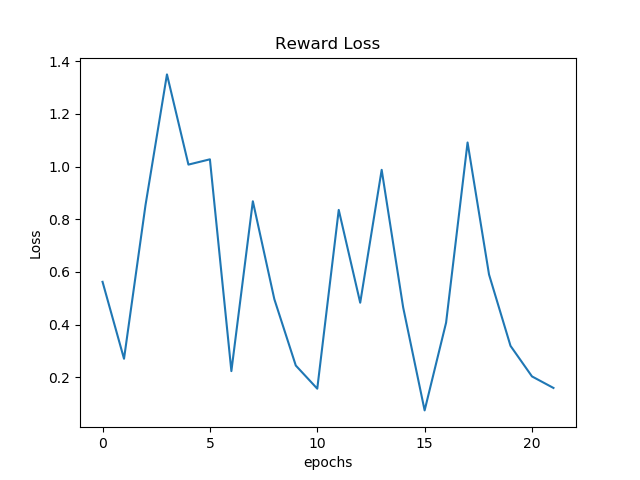
\includegraphics[width=0.45\linewidth]{data/reward_loss01.png} }%
	\subfloat{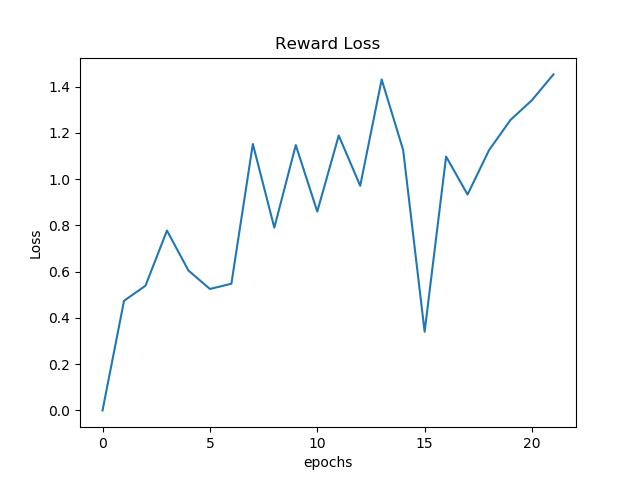
\includegraphics[width=0.45\linewidth]{data/reward_loss05.png} }%
	\caption{Comparison between loss of clips with label $(0,1)$ and $(1,0)$ (on the left) and indifferent labels (on the right).}
	\label{fig:loss0501}%
\end{figure*}
%%%%%%%%%%%%%%%%%%%%%%%%%%%%%%%%%%%%%%%%%%%%%%%%%%%%%%%%%%%%%%%%%%%%%%%%%%%%%%%%%%%%%%%%%%%%%%%

\subsection{Reward Model Loss}
In figure \ref{fig:rewardloss} is shown a particular effect which caught our attention, in essence that the reward loss rises with respect to the increase of the iterations number completed by the system. 
For better understanding this phenomenon we analyze the reward loss in two different components: one coming from all the clip labeled with $(0,1)$ and $(1,0)$; the other coming from the "indifferent labels", that are labeled with $(0.5,0.5)$. You can see the loss plot of the two components in Figure \ref{fig:loss0501}, the left one referred to images with label $(0,1)$ or $(1,0)$ and in the right one the "indifferent labels" loss.
These plots show the loss referred to a training process of 25 iterations for the reward model. 
%Here we split the reward loss in two different components: one coming from all the clip labeled with $(0,1)$ and $(1,0)$; the other coming from the "indifferent labels", that are labeled with $(0.5,0.5)$.
As we can observe from these plots, the losses from the $(0,1)$-$(1,0)$ preferences got a almost fixed range of values, $(0.2,1.4)$, while the ones computed from the "indifferent labels" yield increasing contributions to the overall reward model loss. 
This fact occurs for two main reasons: the number of the "indifferent labels" grows during the training process of the system and for reasons related to the definition of the reward loss function. 
The former is because, since the agent learns how to behave in the environment, after some epochs there are a lot of generated clips with agent steps in the right trajectory, that will be annotated with label $(0.5,0.5)$, so also the number of those "indifferent labels" in the annotation buffer will increase.
The latter comes directly from the definition of the reward loss function reported in section \ref{method} in equation \ref{eq:rewardloss}. The more the reward is accurate, the more $log(\hat{P}[\sigma^i \succ \sigma^j])$ will be close to $\mu(i)$, like every log-loss. When $\mu=(0,1)$ or $\mu=(1,0)$ one of the two terms of the sum will be 0 and the other very close to 1, in essence that will produce a loss almost 0. This does not happen if $\mu=(0.5,0.5)$, where both components of the loss function are non-zero and close to 0.5, which logarithm is not negligible value. For this reason computing the loss for pairs of clips with these labels will make the loss grown during the training protocol. 



\subsection{Resulting Configuration}

Our best configuration produces an agent that performs at every episode the "forced trajectory" both if we sampled actions from a Categorical distribution where logits are the output of the policy model, and if we use a greedy policy. Here the agent will compute always the action with the higher probability, that is an useful approximation when there is a higher action entropy. More in details we set the training protocol epochs to 80, the policy episodes to 150 and K to 1500; policy model has $0.0001$ of learning rate, while the reward model $0.0003$; the annotation are made by a sparse Oracle; after 25 epochs we stop the reward model training. This configuration is reported in Table \ref{table:config}. In Figure\ \ref{fig:rewardloss} and in Figure\ \ref{fig:losspolicy} we report the policy and the reward model loss of this configuration.

%%%%%%%%%%%%%%%%%%%%%%%%%%%%%%%%%%%%%%%%%%%%%%%%%%%%%%%%%%%%%%%%%%%%%%%%%%%%%%%%%%%%%%%%%%%%%%%
\begin{table}[h!]
    \centering
    \begin{tabular}{ |c|c|c|c| } 
        \hline
        \textbf{IRL Component} & \textbf{Parameter} & \textbf{Value} \\
          \hline
          \multirow{5}{*}{\textit{Policy}} & len episode & 150 \\ 
          & \# episodes & 150 \\ 
          & lr  & 0.0001 \\ 
          & std  & 0.5 \\
          & \# rewards & 300 \\
          \hline
          \multirow{2}{*}{\textit{Oracle}} & sparse & (-) \\ 
          & len clip & 5 \\
          \hline
          \multirow{3}{*}{\textit{Reward}} & K & 1500 \\ 
          & lr & 0.0003 \\ 
          & early stopping & 25 it. \\ 
          \hline
    \end{tabular}
    \label{table:config}
\end{table}
%%%%%%%%%%%%%%%%%%%%%%%%%%%%%%%%%%%%%%%%%%%%%%%%%%%%%%%%%%%%%%%%%%%%%%%%%%%%%%%%%%%%%%%%%%%%%%%

To test the reward model accuracy we used the reward model heat map, which is reported in Figure\ \ref{fig:heatmap}. The heat map represents the normalized rewards of all the possible states of the agent. In particular for each Minigrid cell, we take the maximum reward predicted by the reward model between the four possible orientations that the agent can assume and we normalize the resulting values. 
With this heat map we show how the reward model learns to assign higher rewards for those states in the "forced" direction, and lower ones to the other agent positions. The goal state has a small reward, that is because the reward model processes few goal state observations and because the agent episode ends immediately when he reaches this state. Another aspect to take in account is that the states in the fourth column of the heat map have a high reward, even if they do not correspond to the state of the forced trajectory. When the agent is facing up in one of the fourth column states, the Minigrid environment gives the same representation of that where the agent looks down in one of the first column states. For this reason, the reward model predicts similar reward for these symmetric states. 

          % Nicco 

%%%%%%%%%%%%%%%%%%%%%%%%%%%%%%%%%%%%%%%%%%%%%%%%%%%%%%%%%%%%%%%%%%%%%%%%%%%%%%%%%%%%%%%%%%%%%%%
\begin{figure}[t!]
    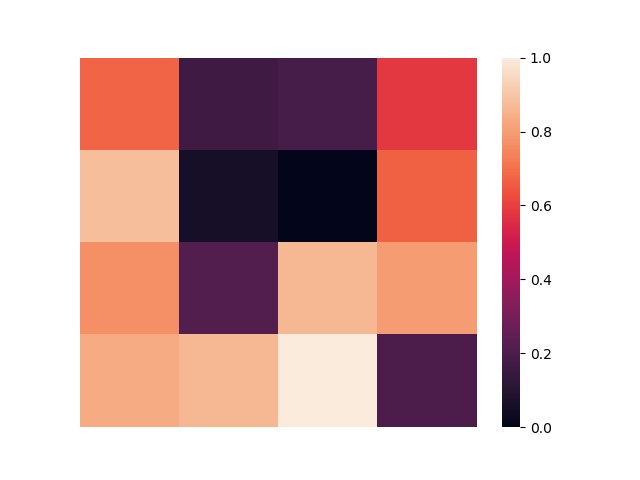
\includegraphics[width=\linewidth]{data/max_heatmap.png} 
    \caption{Heat map that shows the max reward provided from the reward model to the policy. That is computed after the reward model early stop.}
	\label{fig:heatmap}%
\end{figure}
%%%%%%%%%%%%%%%%%%%%%%%%%%%%%%%%%%%%%%%%%%%%%%%%%%%%%%%%%%%%%%%%%%%%%%%%%%%%%%%%%%%%%%%%%%%%%%%

\section{Conclusions}
The aim of this project is to verify the effectiveness of the proposed method by \textit{Borja Ibarz et all.}\ \cite{NIPS2018_8025}, without the human demonstrations. The aim of our project is to force the agent to learn a sub optimal trajectory in the Minigrid environment. This is achieved using the Inverse Reinforcement Learning method: the agent does not take the reward from the environment but there is a reward model that predicts this from agent observations. 

So we define an architecture able to train the agent following our "forced trajectory". Thanks to this, the reward model learns to give high reward to the agent when he is in the forced trajectory states and small reward when the agent is in other states.

The experiments have been carried out in the Minigrid empty environment 6x6, but we believe that this system will work with all the other environment. In particular, the more complex the environments will be, the greater the benefits of the usage of an IRL system will be. This is because in complex environment, the agent will reach the goal state easily using rewards given by a reward model, instead of by the environment. This will reduce the training time, because the agent will not do initial random actions, but he will mimics the human expert behaviour. 
So the user can control step by step what the agent learns from the environment, expressing what the agent has to do in the environment.      

\bibliographystyle{unsrt}
\bibliography{biblio.bib}

\end{document}
